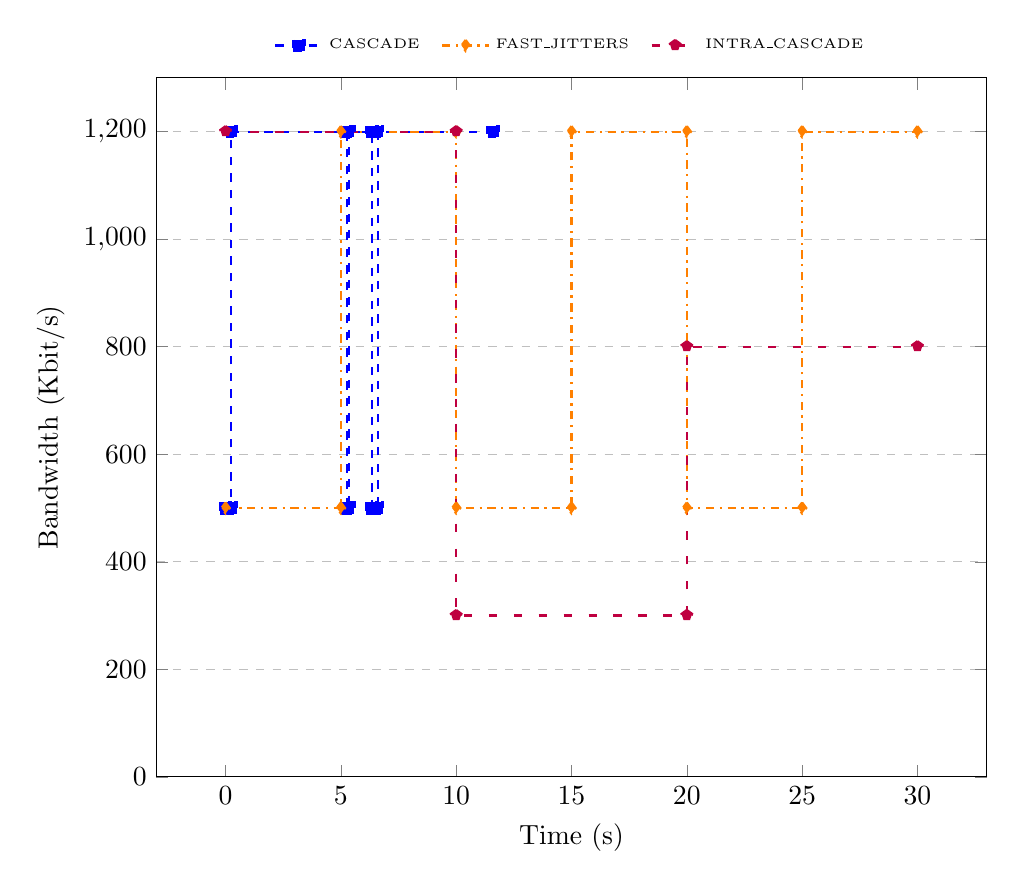
\begin{tikzpicture}
    \begin{axis}[
        width=\textwidth,
        xlabel={Time (s)},
        ylabel={Bandwidth (Kbit/s)},
        ymin=0, ymax=1300, ytick distance=200,
        ymajorgrids=true,
        grid style=dashed,
        legend style={
            at={(0.5,1.02)},
            anchor=south,
            legend columns=-1,
            /tikz/every even column/.append style={column sep=0.2cm},
            font=\tiny,
            draw=none,
            fill=none,
        },
            legend cell align={left},
    ]

% FAST_JITTERS
\addplot[blue, const plot, thick, dashed, mark=square*] coordinates {
    (0,500) (0.25,500) (0.25,1200) (5.25,1200) (5.25,500) (5.35,500)
    (5.35,1200) (6.35,1200) (6.35,500) (6.6,500) (6.6,1200) (11.6,1200)
};

% SLOW_JITTERS
\addplot[orange, const plot, thick, dashdotted, mark=diamond*] coordinates {
    (0,500) (5,500) (5,1200) (10,1200) (10,500) (15,500) (15,1200) (20,1200)
    (20,500) (25,500) (25,1200) (30,1200)
};

% SPIKE
\addplot[purple, const plot, thick, loosely dashed, mark=pentagon*] coordinates {
    (0,1200) (10,1200) (10,300) (20,300) (20,800) (30,800)
};
    
    \legend{CASCADE, FAST\_JITTERS, INTRA\_CASCADE, SLOW\_JITTERS, SPIKE}
    
    \end{axis}
\end{tikzpicture}